\chapter{Background}
\label{ch:background}

% \section{Treatment of children and youth -- the current situation}
% \label{sec:treatment}

% \subsection{The Children and Youth Clinic}

\section{Guideline pathways}
\label{sec:pathways}

National guideline pathways, in Norwegian \emph{pakkeforløp}, are a relatively new thing in the Norwegian health sector. These are standardized ways of treatment and are politically initiated to ensure increased predictability, safety and participation for patients \parencite{helsedirektoratet2019}. They may be for a specific diagnosis and for general use depending on the circumstances. The guideline pathway for mental health and intoxication was introduced in \printdate{2018-09-12} at Nasjonal lanseringskonferanse \parencite{haugland2018} and new patients would be eligible for treatment from \printdate{2019-01-01} onwards. This pathway is then specialized towards adults, children and intoxication respectively. % This project focuses on the guideline pathway for mental health for children and youth.

% Figur av pakkeforløp (uten implementeringsdetaljer)
\begin{figure}
    \centering
    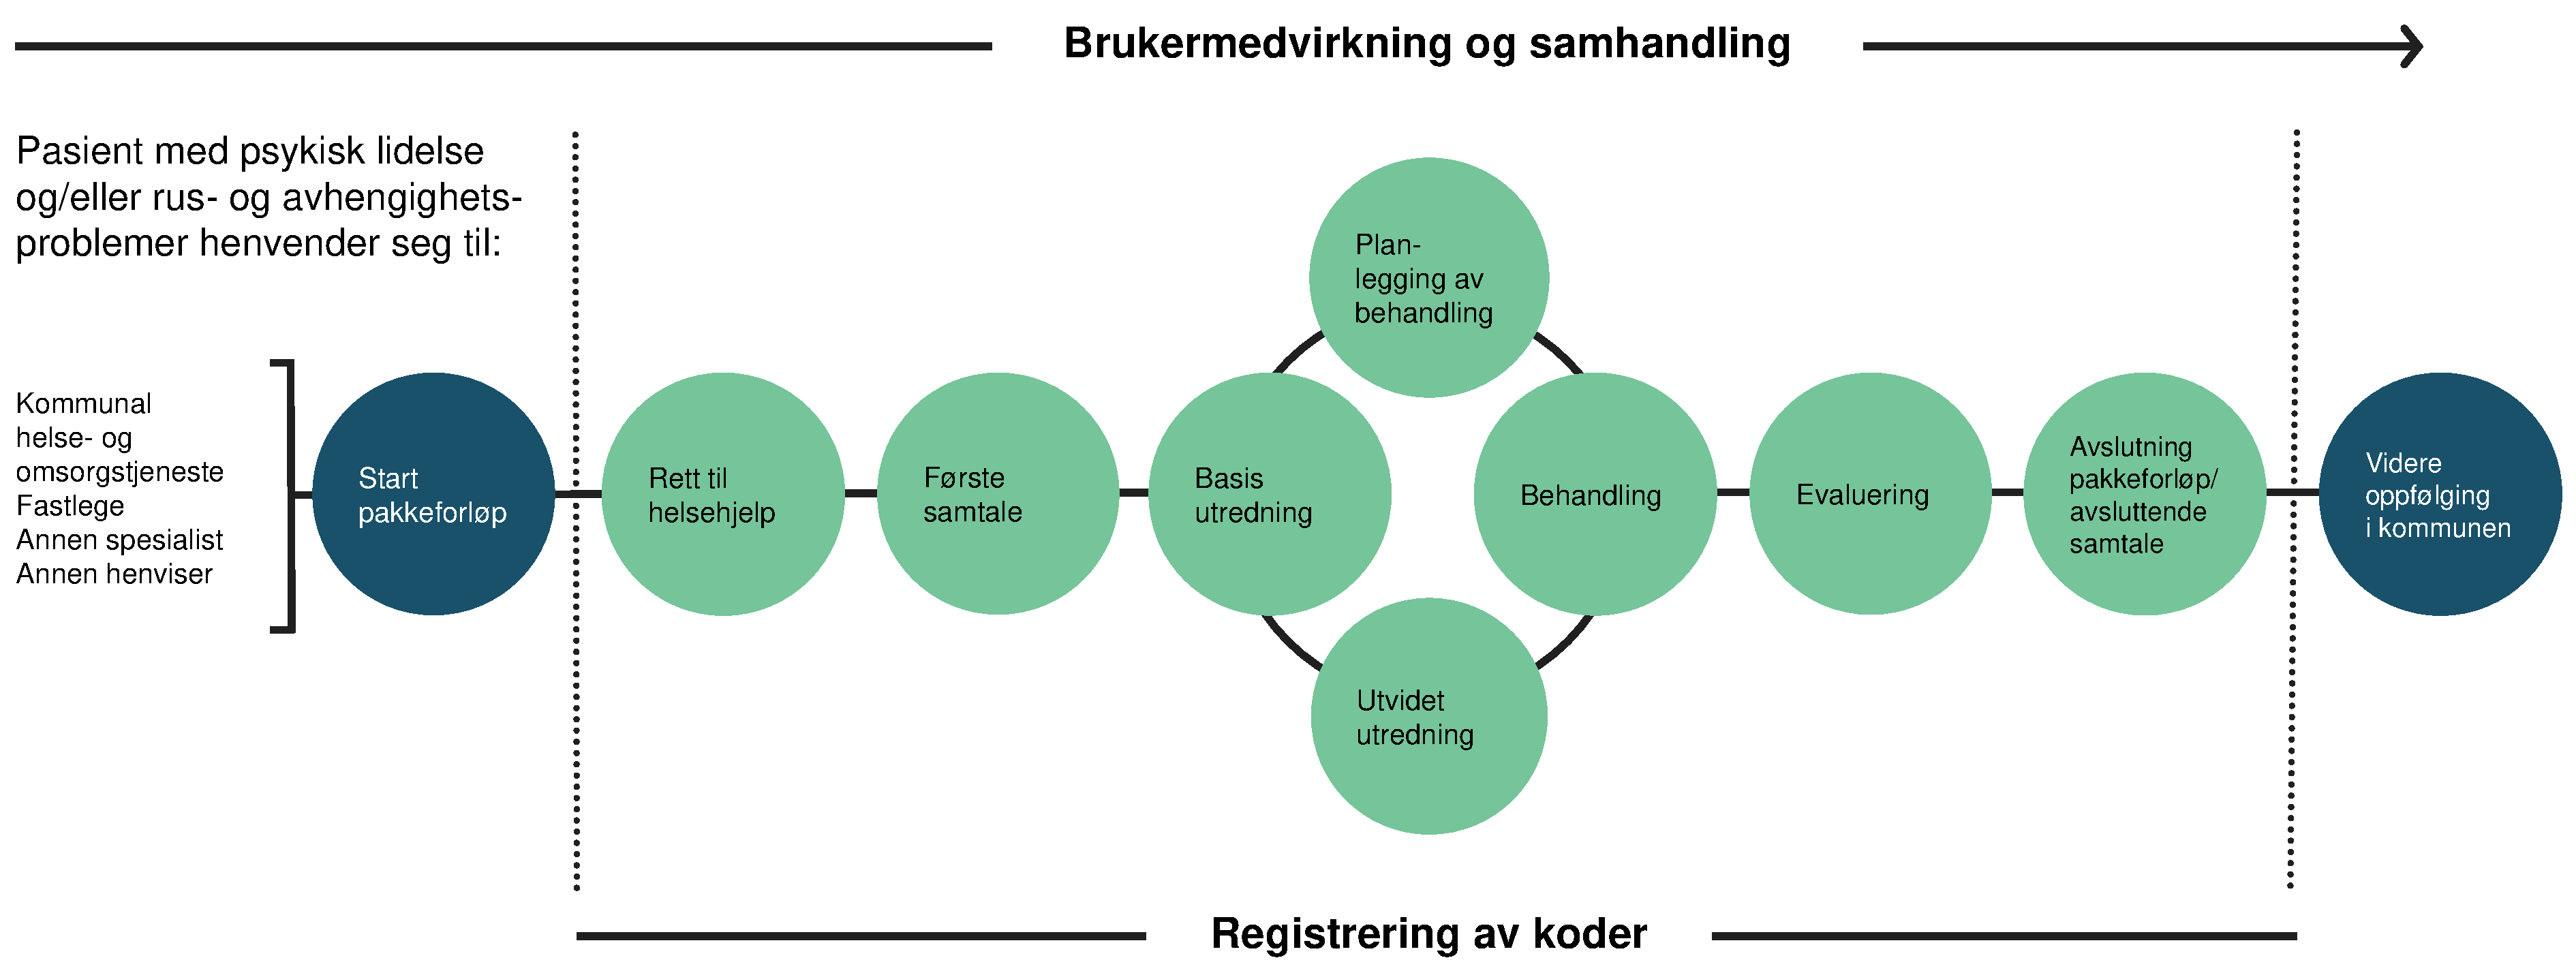
\includegraphics[width=0.9\textwidth]{guideline-pathway.pdf}
    \caption{Guideline pathway for mental health and intoxication}
    Image from \textcite{haugland2018}
    \label{fig:guideline-pathway}
\end{figure}

Guideline pathways are centered around the period of hospitalization, that is, from consultation to discharge. Each pathway consists of a set of phases in a given order. For the guideline pathway for mental health and intoxication, the first steps involves clarifying the needs and goals for the treatment. Then, an inquiry will result in an assessment determining what kind of treatment is the most suitable. This is done in cooperation with the patient. Then follows the treatment which is constantly evaluated to ensure the treatment is working. Lastly, considerations about what needs to be done after the inpatient treatment are made. Some phases have a deadline associated with them, meaning that said phase may not take longer than a certain time to ensure the treatment is done in a timely manner.

\section{Problem areas}
\label{sec:problemareas}

The Children and Youth Clinic stated that they want to improve the ways of which children are informed about upcoming procedures. One of the areas to improve upon is the communication between children and health care services together with its staff. Patients and their relatives have a need for practical information about their treatment while health care services have a need for knowledge about the patient's wishes and feedback. If this communication is problematic, or there is a lack thereof, patients may start to miss out on information and feel excluded from the decision-making. Use of medical terminology without explanation can contribute to this exclusion \parencite{coyne2006}.

Another related issue is that the information that is handed out at hospitals is often not personalized. This includes paper documents, brochures, web pages, internal systems among others. Currently, the information that is given here is primarily textual and of varying interest for younger patients. When this information lacks personalization, there is an increased chance that patients---especially younger ones---will miss out on details, not be motivated and not engage in their treatment.

Comics and cartoon drawings may work as a measure against both problem areas. It is shown that cartoon illustrations help to make instructions easier to grasp and make sense of \parencite{delp1996}. This may be combined with personalization as seen in \emph{E-LAN} (see \autoref{sec:relatedwork}) -- where the comic character is replaced with a patient's respective avatar. Doing this, the anticipation is that patients may find themselves in the situation, rather than seeing someone they don't associate with.

% This bottoms out into fundamental rights 
% In a report from the Norwegian Institute of Public Health, \textcite{norwegianinstitute2015} (...)
% Children should be enabled to express their views and participate in decisions regarding their treatments \parencite{coyne2006}.

\section{Preceding projects}

This project builds upon experience from a bachelor thesis named \emph{PictogramApp}, which was based on another project named \emph{Pictogram-me}.

\subsection{Pictogram-me}

Since 2011, associate professor in graphic design Linda Lien and professor in visual communication Ashley Booth have researched on creative usage of pictograms. A pictogram, also called a pictograph, is a simplified figure that resembles and represents a physical object. They vary in shapes and sizes, but they are ultimately designed in a way that make them easy to interpret and understand their symbolic meaning.

Lien's and Booth's artistic research project, named \emph{Pictogram-me}, experiments how pictograms can be used to express complex social messages \parencite{lien2018}. The aim is to illustrate challenging situations that people who have a difficult life may endure. Despite pictograms being flat and simplified, Lien and Booth wanted to show how pictograms also can visualise difficult topics and promote empathy.

Pictogram-me presents a new set of pictograms that are designed for the purpose of the project. In addition, the project has resulted in various concepts including

\begin{itemize}
    \item \emph{PictoBooth}, a photo booth that translates the body and gestures into real life pictograms,
    \item \emph{PictoFont}, a symbol typeface consisting of various pictograms, and
    \item \emph{PictoTheatre}, a small-scale theatre where pictograms can be arranged on a scene. A tablet can be placed behind the scene and function as a background as illustrated in \autoref{fig:pictotheatre}.
\end{itemize}

\begin{figure}
    \centering
    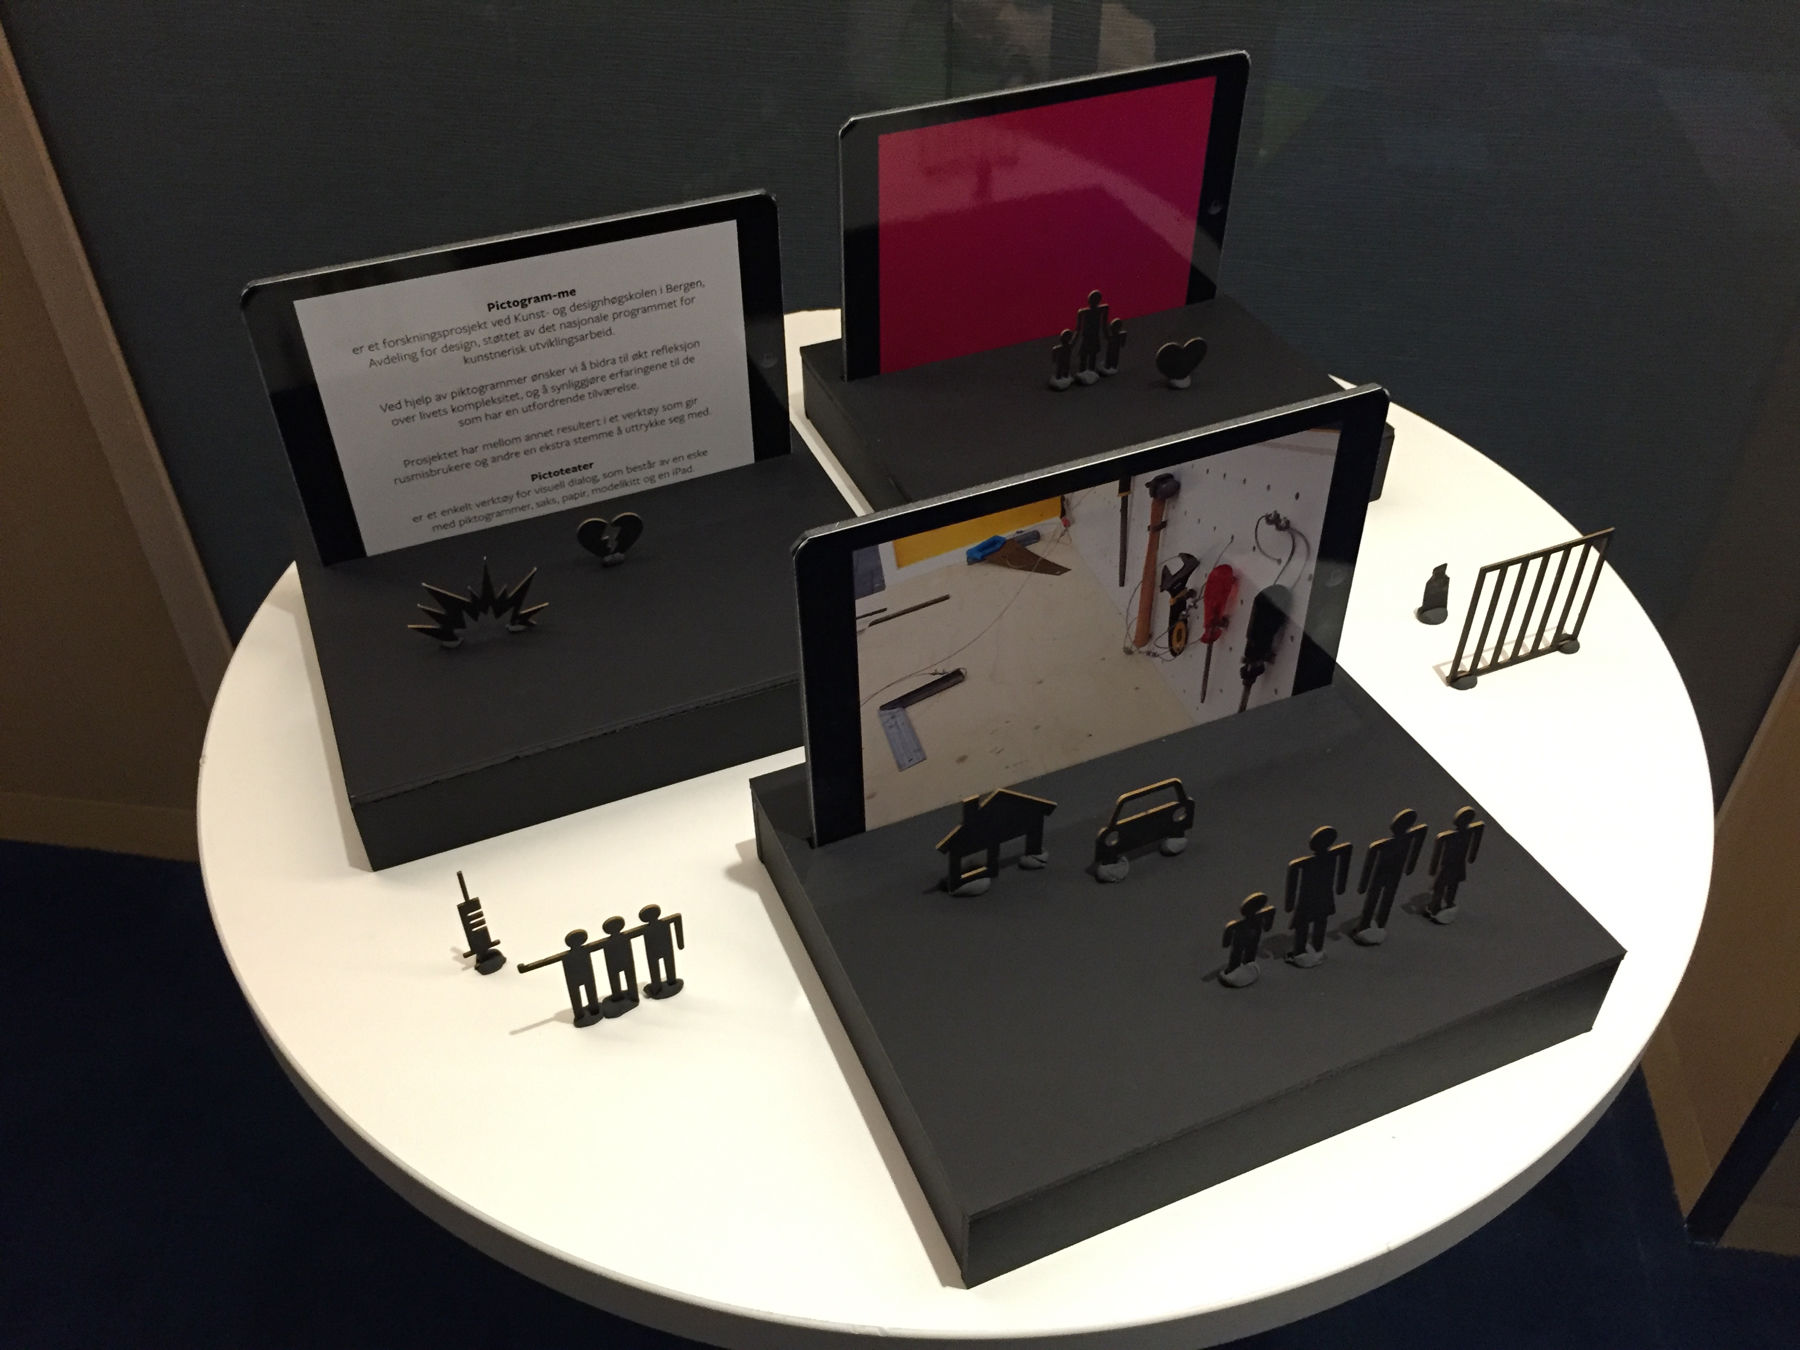
\includegraphics[width=0.75\textwidth]{pictotheatre.jpg}
    \caption{PictoTheatre, shown at the 2016 RØST conference in Bergen}
    Photograph by \textcite{lien2018}
    \label{fig:pictotheatre}
\end{figure}

\subsection{PictogramApp}

In 2017, the Western Norway University of Applied Sciences issued a bachelor project in collaboration with Linda and Booth, with the purpose of creating a smartphone application. The application, which was later named \emph{PictogramApp}, was meant to be a digital version of PictoTheatre where pictograms can be arranged on the screen and form visual messages in a mobile manner \parencite{fure2017}. The application allows users to place pictograms in context in order to create their own stories. Two screenshots from this app are shown in \autoref{fig:pictogramapp}. PictogramApp was targeted towards the Church City Mission, a voluntary organisation which offers help and services for people living near the street. A beta version of the application was released in June 2017.

\begin{figure}
    \centering
    \hspace{\fill}
    \begin{subfigure}{0.31\textwidth}
        \centering
        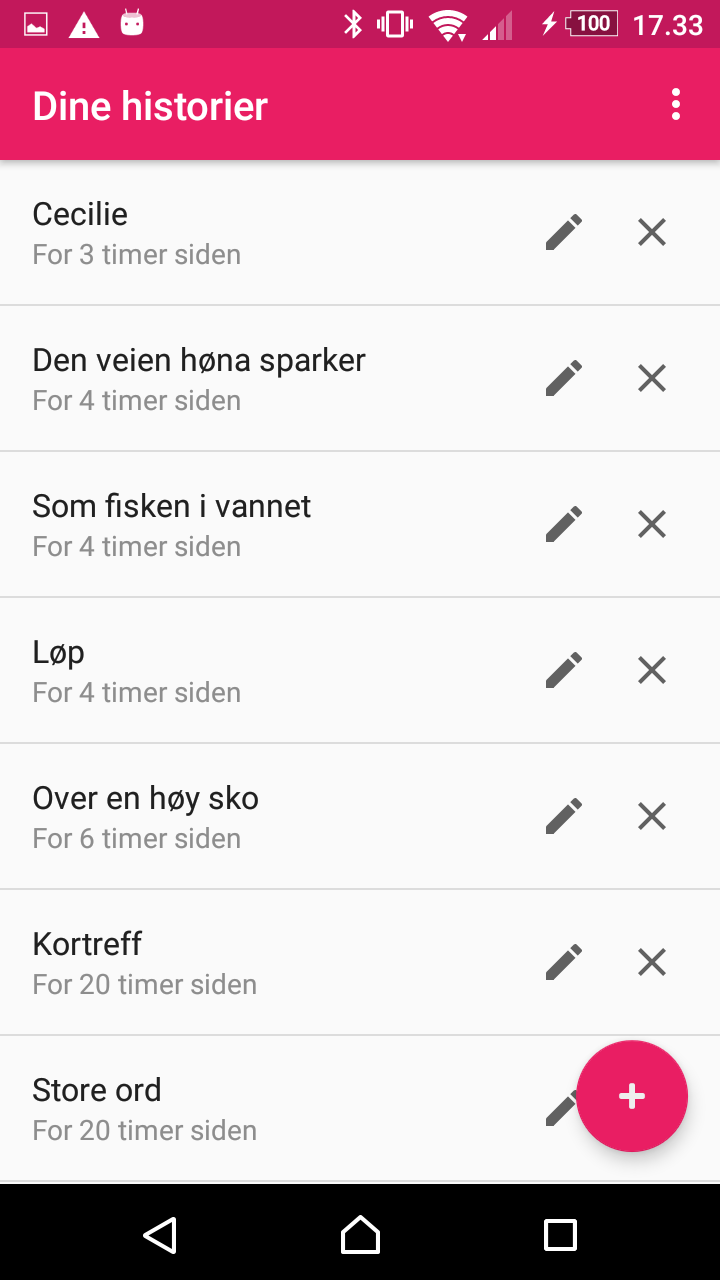
\includegraphics[width=\textwidth]{pictogramapp-01.png}
        \subcaption{List of stories}
        \label{fig:pictogramapp-list}
    \end{subfigure}
    \hspace{\fill}
    \begin{subfigure}{0.31\textwidth}
        \centering
        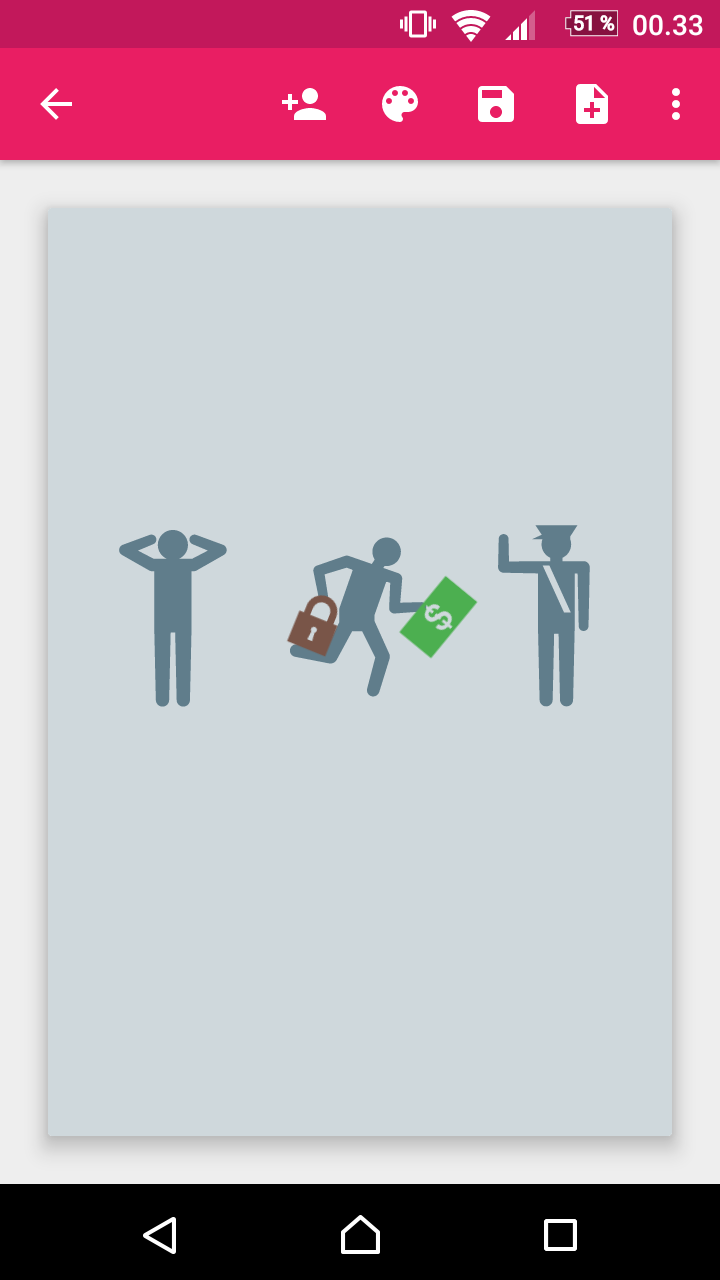
\includegraphics[width=\textwidth]{pictogramapp-02.png}
        \subcaption{Scene editing}
        \label{fig:pictogramapp-scene}
    \end{subfigure}
    \hspace*{\fill}
    \caption{Screenshots from PictogramApp}
    \label{fig:pictogramapp}
\end{figure}

\section{Related work}
\label{sec:relatedwork}

The Children and Youth Clinic has prior to this project experimented with different ways to engage their patients. Among these was a lan party event named \emph{E-LAN} held in October 2018 \parencite{helsebergen2018}. The purpose of this event was to connect gaming towards a healthy lifestyle and to let children and youth find a sense of achievement in new areas. As a part of this initiative, an avatar generation system was created by Helse Vest IKT that lets users create personal avatars which represent themselves. These would be printed onto physical name tags of which children and youth could attach on their clothings and carry with them. The avatars did not necessarily reflect their visual appearance, though they could be immediately recognized by their respective owner.

In order to discover related work and gain further insight in the problem area, a set of queries were performed on academic literature search engines. Each query contained a set of the following keywords:

\begin{multicols}{3}
    \raggedcolumns
    \begin{itemize}
        \item Hospital
        \item Patient
        \item Pediatric
        \item Children
        \item Information
        \item Informative
        \item Interactive
        \item Understanding
        \item Comprehension
        \item Engage
        \item Cartoon
        \item Comics
        \item Illustrations
        \item Personalised
    \end{itemize}
\end{multicols}

% List relevant papers that cover the problem area?

Several applications and prototypes have been made that aim to provide information about and illustrate a child's hospital stay. A notable example is \emph{IACTA}, short for \emph{Inter-Active Communication Tool for Activities}. This application was co-designed together with children \parencite{stalberg2016} and then analysed as children used the application \parencite{stalberg2018}. Another example is an inpatient portal application named \emph{MyChart Bedside}, developed by Epic Systems Corporation for tablet devices. The application shows a calendar, a list of diagnoses to be treated, a list of medications and lab results. The portal was shown to be well received by children's parents \textcite{kelly2017}. A third example is by \textcite{maher2016}, a tool visualizing a roadmap interface on a tablet device. The roadmap is a metaphor of the hospital stay, consisting of several phases that make up the hospitalization period.

Literature about communication with hospitalized children is growing. The topic of consultation with children and their participation in decision-making has been investigated in \textcite{coyne2006,coyne2008,coyne2011}. Throughout consultations, a literature review and interviews respectively, the findings indicate a lack of participation and engagement for the children. These papers have a unified experience that children's views are rarely taken into consideration, often neglected in favour of communication with the parents instead. Sometimes this is what the child wants, as \textcite{lambert2011} says that health professionals identified children as either passive bystanders or active participants. This has a direct consequence of the child's participation in communication.

Medical procedures may be looked upon as step-by-step instructions that should be replicated. Public instructions are plentiful, but for brevity, an example to consider is one used by Norwegian Airline Systems on their aeroplanes. Instead of paying attention to the cabin crew who demonstrates the use of safety gadgets and emergency procedures, an animated video \parencite{norwegianairshuttle2012} is shown for the passengers. This animation depicts a child and their parent as they go through each procedure. Not only does this provide visual information that the cabin crew cannot show on their own; children and parents may identify themselves as the characters in the video, attracting further attention.

\begin{figure}
    \centering
    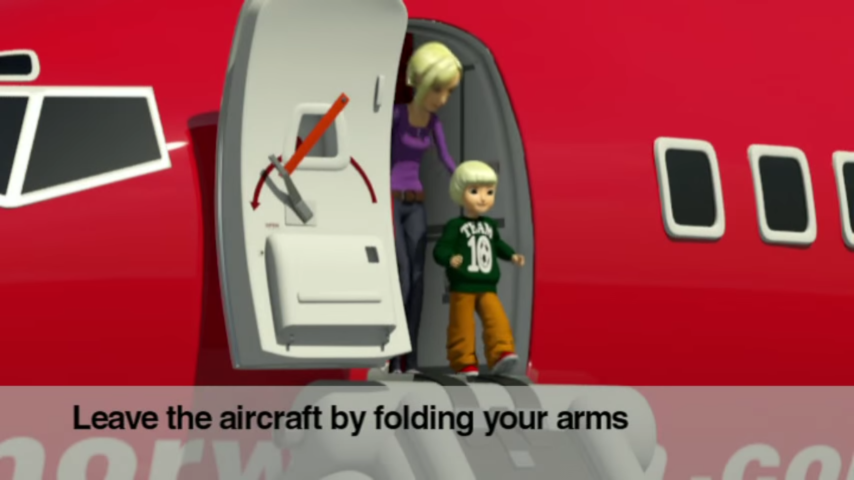
\includegraphics[width=0.7\textwidth]{safetyonboard.png}
    \caption{Snapshot of the instruction video \enquote{Safety onboard}}
    Video produced by Skyline IFE
    \label{fig:safetyonboard}
\end{figure}

Another step in increased personalization is the use of personal avatars, where a user may create a character that represents themselves. Herein lies several examples as well, the most popular one being Bitmoji. Bitmoji is an integrated app in the popular social media platform Snapchat that features personalized cartoon avatars for their users. It is a spin-off of Bitstrips.com, a web application that was more focused on comic strips designed for educational use. % Blackstock and Brown, two of the founders, (...)
